\section{Analyse des données}

\begin{frame}
  \frtt{Analyse des données}
\textbf{Source} :\\
	\begin{itemize}
		\item VLBI Earth Orientation Solution OPA2015a	
		\item Rigid Earth Nutation (Souchay et al. 1997)
	\end{itemize}
\textbf{Données} :
	\begin{itemize}
	\item séries temporelles de nutations en $X(t)$ et $Y(t)$
	\end{itemize}
	\vfill
	\onslide<2->{
	Ajustement des amplitudes complexes $\widetilde{A} = A_{Re} + iA_{Im}$ par méthode des moindres carrés :
	\begin{equation*}
	\left(X+ iY\right) = \sum\limits_{j=1}^{40} (\widetilde{A}_{j} \times e^{(\omega_{j}*t + \varphi_{j})})
	\only<3>{+ \tilde{a}t + \tilde{b}}
	\end{equation*}

%	$\widetilde{A}$ : amplitude \\
%	$\omega$ : fréquence \\
%	$\varphi$ : phase \\
%	$t$ : temps
}
\end{frame}

\begin{frame}
  \frtt{Amplitudes Ajustées}
	\begin{center}
		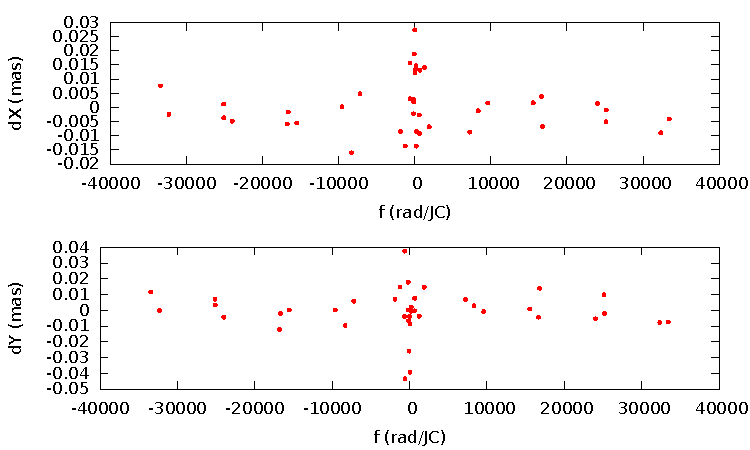
\includegraphics[width=1.0\textwidth]{amplitude_freq.pdf}
	\end{center}
\end{frame}

\begin{frame}
  \frtt{Corrélations}
  \centerline{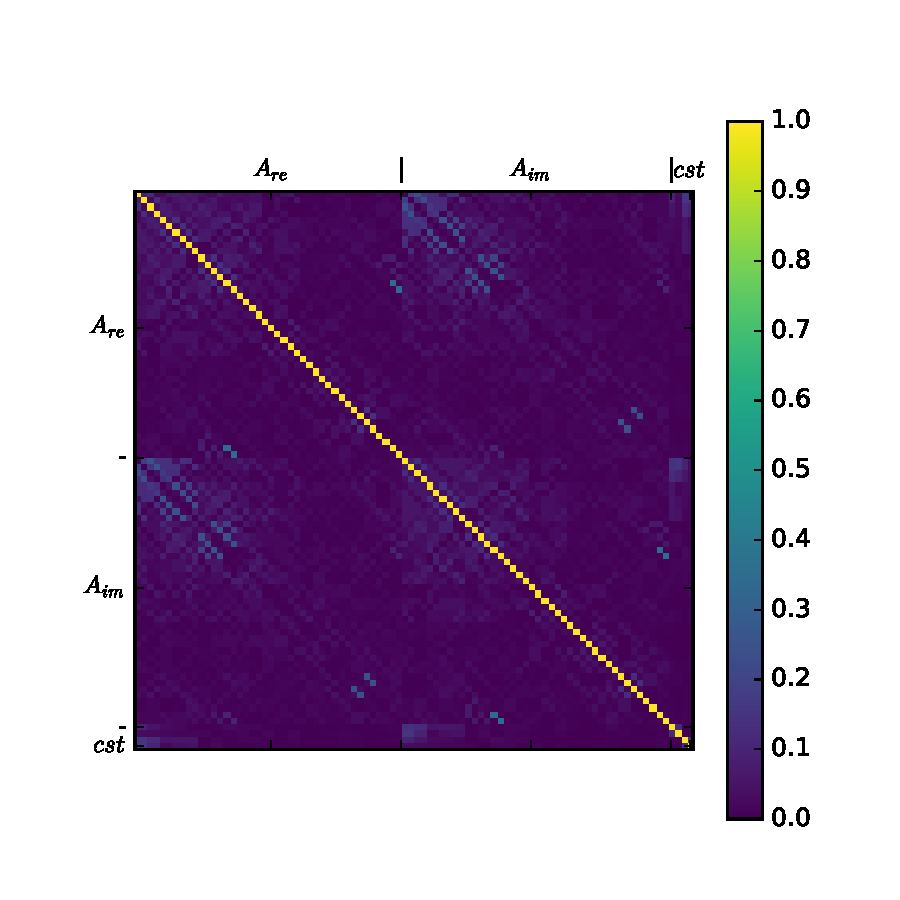
\includegraphics[width=0.8\textwidth]{fit_amplitude_correlation.pdf}}
\end{frame}


\begin{frame}
  \frtt{Série ajustée VS observations}
	\begin{center}
		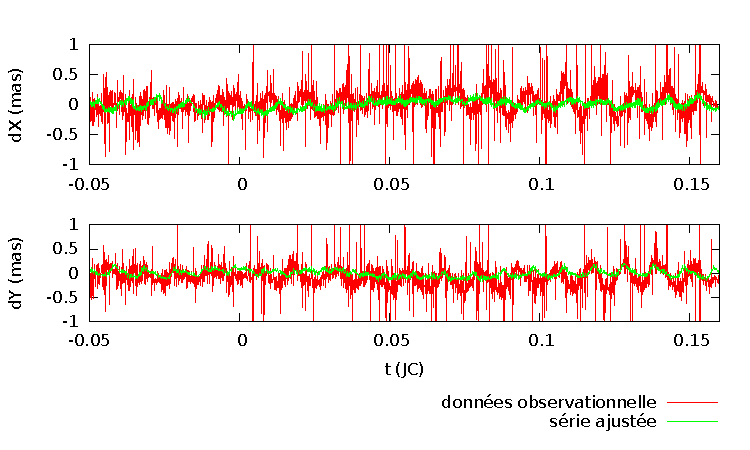
\includegraphics[width=1.0\textwidth]{fit_amplitude_ser_obs.pdf}
	\end{center} 
\end{frame}

